\documentclass[11pt,a4paper,twoside]{tesis}
% SI NO PENSAS IMPRIMIRLO EN FORMATO LIBRO PODES USAR
%\documentclass[11pt,a4paper]{tesis}

\usepackage{graphicx}
\usepackage{float}
\usepackage[utf8]{inputenc}
\usepackage[spanish,es-noquoting]{babel}
\usepackage[left=3cm,right=3cm,bottom=3.5cm,top=3.5cm]{geometry}
\usepackage{amsmath}
\usepackage{amssymb}
\usepackage{tikz}
\usepackage{subcaption}
\usetikzlibrary{arrows.meta}

\begin{document}

%%%% CARATULA

\def\autor{Ignacio Fernández Oromendia}
\def\tituloTesis{Optimizaci\'on de recorridos para la recolecci\'on de reciclables}
\def\runtitulo{Optimizaci\'on de recorridos para la recolecci\'on de reciclables}
\def\runtitle{Optimizing routes for recyclable collection}
\def\director{Paula Zabala}
\def\codirector{Isabel Mendez Díaz}
\def\lugar{Buenos Aires, 2025}
\newcommand{\HRule}{\rule{\linewidth}{0.2mm}}
%
\thispagestyle{empty}

\begin{center}\leavevmode

\vspace{-2cm}

\begin{tabular}{l}

\includegraphics[width=2.6cm]{logofcen.pdf}
\end{tabular}


{\large \sc Universidad de Buenos Aires

Facultad de Ciencias Exactas y Naturales

Departamento de Computaci\'on}

\vspace{6.0cm}

%\vspace{3.0cm}
%{
%\Large \color{red}
%\begin{tabular}{|p{2cm}cp{2cm}|}
%\hline
%& Pre-Final Version: \today &\\
%\hline
%\end{tabular}
%}
%\vspace{2.5cm}

\begin{huge}
\textbf{\tituloTesis}
\end{huge}

\vspace{2cm}

{\large Tesis de Licenciatura en Ciencias de la Computaci\'on}

\vspace{2cm}

{\Large \autor}

\end{center}

\vfill

{\large

{Directora: \director}

\vspace{.2cm}

{Codirectora: \codirector}

\vspace{.2cm}

\lugar
}

\newpage\thispagestyle{empty}


%%%% ABSTRACTS, AGRADECIMIENTOS Y DEDICATORIA
\frontmatter
\pagestyle{empty}
%\begin{center}
%\large \bf \runtitulo
%\end{center}
%\vspace{1cm}
\chapter*{\runtitulo}

TODO

\bigskip

\noindent\textbf{Palabras claves:} Guerra, Rebelión, Wookie, Jedi, Fuerza, Imperio (no menos de 5).

\cleardoublepage
%\begin{center}
%\large \bf \runtitle
%\end{center}
%\vspace{1cm}
\chapter*{\runtitle}

\noindent In a galaxy far, far away, a psychopathic emperor and his most trusted servant -- a former Jedi Knight known as Darth Vader -- are ruling a universe with fear. They have built a horrifying weapon known as the Death Star, a giant battle station capable of annihilating a world in less than a second. When the Death Star's master plans are captured by the fledgling Rebel Alliance, Vader starts a pursuit of the ship carrying them. A young dissident Senator, Leia Organa, is aboard the ship \& puts the plans into a maintenance robot named R2-D2. Although she is captured, the Death Star plans cannot be found, as R2 \& his companion, a tall robot named C-3PO, have escaped to the desert world of Tatooine below. Through a series of mishaps, the robots end up in the hands of a farm boy named Luke Skywalker, who lives with his Uncle Owen \& Aunt Beru. Owen \& Beru are viciously murdered by the Empire's stormtroopers who are trying to recover the plans, and Luke \& the robots meet with former Jedi Knight Obi-Wan Kenobi to try to return the plans to Leia Organa's home, Alderaan. After contracting a pilot named Han Solo \& his Wookiee companion Chewbacca, they escape an Imperial blockade. But when they reach Alderaan's coordinates, they find it destroyed - by the Death Star. They soon find themselves caught in a tractor beam \& pulled into the Death Star. Although they rescue Leia Organa from the Death Star after a series of narrow escapes, Kenobi becomes one with the Force after being killed by his former pupil - Darth Vader. They reach the Alliance's base on Yavin's fourth moon, but the Imperials are in hot pursuit with the Death Star, and plan to annihilate the Rebel base. The Rebels must quickly find a way to eliminate the Death Star before it destroys them as it did Alderaan (aprox. 200 palabras).

\bigskip

\noindent\textbf{Keywords:} War, Rebellion, Wookie, Jedi, The Force, Empire (no menos de 5). % OPCIONAL: comentar si no se quiere

\cleardoublepage
\chapter*{Agradecimientos}

\noindent Lorem ipsum dolor sit amet, consectetur adipiscing elit. Fusce sapien ipsum, aliquet eget convallis at, adipiscing non odio. Donec porttitor tincidunt cursus. In tellus dui, varius sed scelerisque faucibus, sagittis non magna. Vestibulum ante ipsum primis in faucibus orci luctus et ultrices posuere cubilia Curae; Mauris et luctus justo. Class aptent taciti sociosqu ad litora torquent per conubia nostra, per inceptos himenaeos. Mauris sit amet purus massa, sed sodales justo. Mauris id mi sed orci porttitor dictum. Donec vitae mi non leo consectetur tempus vel et sapien. Curabitur enim quam, sollicitudin id iaculis id, congue euismod diam. Sed in eros nec urna lacinia porttitor ut vitae nulla. Ut mattis, erat et laoreet feugiat, lacus urna hendrerit nisi, at tincidunt dui justo at felis. Class aptent taciti sociosqu ad litora torquent per conubia nostra, per inceptos himenaeos. Ut iaculis euismod magna et consequat. Mauris eu augue in ipsum elementum dictum. Sed accumsan, velit vel vehicula dignissim, nibh tellus consequat metus, vel fringilla neque dolor in dolor. Aliquam ac justo ut lectus iaculis pharetra vitae sed turpis. Aliquam pulvinar lorem vel ipsum auctor et hendrerit nisl molestie. Donec id felis nec ante placerat vehicula. Sed lacus risus, aliquet vel facilisis eu, placerat vitae augue.
 % OPCIONAL: comentar si no se quiere

\cleardoublepage
\hfill \textit{A mi persona favorita.}
  % OPCIONAL: comentar si no se quiere

\cleardoublepage
\tableofcontents

\mainmatter
\pagestyle{headings}

%%%% ACA VA EL CONTENIDO DE LA TESIS

\chapter{Introducción}
\section{Contexto}

La provincia de Buenos Aires es una de las zonas más pobladas de la Argentina, con una significativa producción de residuos urbanos. Esto hace que la gestión de residuos reciclables represente un desafío crucial para los municipios, que buscan implementar sistemas eficientes y sostenibles para el reciclaje. 

\vspace{3mm}

Mediante programas de educación y concientización se ha logrado fomentar la separación en origen, donde los ciudadanos separan los residuos reciclables de los no reciclables en sus hogares. Para complementar esta tarea, algunos municipios de la provincia han implementado la recolección de residuos reciclables por medio de sistemas puerta a puerta, mediante camiones que recorren sus calles de forma semanal, un día específico según la zona del municipio. Estos camiones recogen los residuos de las puertas de los hogares y los llevan a una planta de clasificación, donde los materiales reciclables se separan y procesan. 

\vspace{3mm}

En el caso de San Isidro, el municipio decidió separar su terreno en 6 zonas distintas siguiendo la idea de las separación barrial. Estas zonas son: Acassuso, Beccar, Boulogne, Martínez, San Isidro y Villa Adelina. Para no alterar la rutina de los vecinos no se van a modificar estas zonas, por lo cual vamos a resolver el problema de optimización para cada una de ellas por separado.

\vspace{3mm}

El servicio consiste en que uno o varios camiones recorren las calles de cada
zona el día determinado por el municipio, recogiendo las bolsas dejadas por los
vecinos. Cuando la capacidad del camión es alcanzada, la recolección realizada
hasta ese momento es llevaba a una planta de clasificación. Si fuera necesario,
los camiones realizan más de un viaje diario.

\vspace{3mm}

El desarrollo realizado por el Departamento de Computación de la Facultad de
Ciencias Exactas de la Universidad de Buenos Aires tuvo como objetivo encontrar diferentes alternativas de recorridos que contemplan diversos objetivos y restricciones.

\section{Definiciones}

Un \textit{grafo} $G$ consiste en un par $G = (V,E)$ donde $V$ es un conjunto vértices y $E$ es un conjunto de pares $(v,u)$ las cuales llamaremos aristas. Estos pares son bidireccionales, es decir, podemos ir desde $v$ a $u$ y viceversa. Por otro lado, tenemos los \textit{grafos dirigidos} $D$, los cuales también consisten en un par $D = (V,E)$ que representan lo mismo que en un grafo salvo que en este caso, los pares $(v,u)$ de $E$ no son bidireccionales. Estos tienen la dirección igual a la de su par, podemos ir de $v$ a $u$ pero no podemos hacer la inversa.

\vspace{3mm}

En este problema vamos a trabajar con un \textit{grafo mixto} $G$ el cual contiene ambos tipos de ejes. Es decir, $G = (V, E\cup A)$ donde $E$ contiene las aristas bidireccionales y $A$ las aristas unidireccionales, las cuales llamaremos arcos.

\section{Problemas de recorrido}

No se puede poner una fecha de origen [CAMBIAR ORIGEN] para los problemas de recorrido, pero si podemos decir que fueron el punta pie para el origen de la teoría de grafos. El ejemplo clásico es el problema de los puentes de \textbf{Konigsberg} [BUSCAR COMO HACER EL : EN LA O], el cual tiene el nombre de la ciudad a la cual es origen. En esta ciudad tenemos un río que se bifurca y rodea un terreno separando en 4 regiones la ciudad conectada por 7 puentes. El problema consistía en encontrar un recorrido para cruzar a pie toda la ciudad pasando solo una vez por cada uno de los puentes y regresando al mismo punto de inicio. En la actualidad, a este tipo de problemas se lo conoce como circuito euleriano. En el área de optimización combinatoria a este problema se lo conoce como el problema de \textit{cartero chino}

\subsection{Problema del Cartero Chino}

Dada una ciudad con calles e intersecciones, el problema consiste en encontrar el circuito más corto que visite cada calle volviendo al punto de partida. Formalizando el problema del Cartero Chio (CPP), podemos decir que dado un grafo $G = (V,E)$ y una función de costos sobre cada una de las aristas de $E$ queremos determinar un circuito que contenga a todo elemento de $E$ y que la suma de costos de las aristas utilizadas sea mínimo.

\vspace{3mm}

Un aspecto curioso sobre este problema es que sus versiones dirigidas y no dirigida  tienen una complejidad temporal polinomial, es decir, se encuentra en la clase $P$ de problemas, es decir, es posible resolverlo en tiempo razonable y se considera de una baja dificultad. Con lo cual, uno pensaría que su versión mixta también será accesible de resolver. Sin embargo, todo lo contrario, el problema del cartero chino mixto se encuentra dentro de la clase de complejidad $NP$-Completo, con lo cual, no existe algoritmo que en complejidad temporal polinomial lo resuelva.

\vspace{3mm}

No obstante, podemos modelar este tipo de problemas con programación lineal donde tendremos una función objetivo sujeta a restricciones que nos darán la solución óptima al problema. Para resolver este tipo de problema se usa el algoritmo \textit{SIMPLEX}, desarrollado por George Dantzig en 1947, que a traves de analizar los vértices del polígono generado por el modelo y varias iteraciones de procesamiento y reducción del espacio de búsqueda encuentra la solución óptima. \textit{SIMPLEX} tiene una complejidad teórica temporal exponencial, con lo cual nos deja parados fuera de la clase $P$. Sin embargo, en la práctica este alogritmo es polinomial, con lo cual, resulta muy útil para resolver problemas de recorrido.

\subsection{Problema del Cartero Chino Rural}

El problema del Cartero Chino Rural (RPP) nos presenta la misma situación que el su versión original. La diferencia se encuentra en que, dado un grafo mixto $G = (V,E\cup A)$ en este caso vamos a tener un conjunto $R \subseteq E \cup A$ de ejes obligatorios a recorrer. Aunque cambia la dificultad del problema ya que no hace falta recorrer todas los ejes si no que sólo los que contiene $R$, este se encuentra en la clase $NP$-Completo.

\subsection{Capacitated Arc Routing Problem}

Los problemas CARP se originan a partir del problema del Cartero Chino Rural donde se le agregan al problema una función de capacidad, la cual asigna una demanda a cada eje del grafo, y una capacidad al vehículo que la recorre. Esto nos obliga a tener que partir en distintas rutas en caso de que no se pueda recorrer todos los ejes obligatorios cumpliendo con la restricción de capacidad.

\chapter{Optimizando tiempo}
\section{Modelo Inicial}

Algo que introduzca esto

\vspace{3mm}

Dado un grafo $G = (V,E\cup A)$, $R \subseteq E\cup A$ como el conjunto de ejes obligatorios de recorrer,  
$t:E\cup A\rightarrow \mathbb{R}$ como el tiempo en recorrer el eje $ij$, $q:E\cup A\rightarrow \mathbb{R}$ 
como la demanda del eje $ij$ y $W$ la capacidad de cada camión, definimos las siguientes variables.

\begin{align*}
    X^p_{ij} &= 
    \begin{cases}
        1 & \text{si el eje } ij \text{ fue satisfecho en el viaje } p \\
        0 & \text{caso contrario}
    \end{cases} \\
    Y^p_{ij} &= \text{Cantidad de veces que el eje } ij \text{ fue recorrido sin recoger en el viaje } p \\
    F^p_{ij} &= \text{Flujo del eje } ij \text{ en el viaje } p \\
\end{align*}

El modelo que en una primera instancia resuelve el problema es el siguiente. Como notación vamos a usar $t_{ij}$ 
en lugar de $t(ij)$ para referirnos al tiempo en recorrer el eje $ij$, además usaremos $S = E\cup A$.

\begin{align}
    \min \quad & \sum^P_{p=1}(\sum_{ij\in R}t_{ij}X^p_{ij} + \sum_{ij\in S}t_{ij}Y^p_{ij}) \\
    \text{sujeto a} \quad & \sum_{j/ij\in S} Y^p_{ij} + \sum_{j/ji\in R} X^p_{ij} = \sum_{j/ji\in S} Y^p_{ji} + \sum_{j/ij\in R} X^p_{ji} & \forall i \text{ } \forall p \\
    & \sum_{p=1} X_{ij}^p = 1 & \forall ij \in R \cap A \\
    & \sum_{p=1} (X_{ij}^p + X_{ji}^p) = 1 & \forall ij \in R \cap E \\
    & \sum_{j:(0j)\in S} Y^p_{0j} + \sum_{j:(0j)\in R} X^p_{0j} \leq 1 & \forall p \\
    & \sum_{j:(ji)\in S} F^p_{ji} - \sum_{j:(ij)\in R} F^p_{ij} = \sum_{j:(ji)\in R}q_{ij} X_{ji}^P & \forall i \text{ } \forall p \\
    & \sum_{j:(0j) \in S} F^p_{0j} = \sum_{(ij)\in R} q_{ij}X_{ij}^p & \forall i \forall p \\
    & \sum_{i:(i0) \in S} F^p_{i0} = \sum_{i:(i0)\in R} q_{i0}X_{i0}^p & \forall p \\
    & F^p_{ij} \leq W(y^p_{ij} + x^p_{ij}) & \forall(i,j) \in S, \forall p \\
    & X^p_{ij} \in \{0,1\} & \forall(i,j) \in R, \forall p \\
    & F^p_{ij} \geq 0 & \forall(i,j) \in S, \forall p \\
    & Y^p_{ij} \geq 0 \text{ entera} & \forall(i,j) \in S, \forall p
\end{align}

La función objetivo (1) del problema representa el costo total del recorrido, es decir, el costo 
de recoger residuos y el de recorrer por ejes sin recoger. La condición (2) impone continuidad al 
recorrido sobre cada nodo, que todo nodo tenga la misma cantidad de entradas que salidas. 
Luego, (3) y (4), obligan a recorrer todos los arcos y aristas respectivamente. 
En la restricción (5) nos aseguramos de que en cada camión salga del depósito a lo sumo una vez. 
Luego, las condiciones (6)-(9) tienen la función de conservar el flujo y forzar la conectividad entre cada nodo. 
Por otro lado, la condición (9) impone una cota súperior que garantiza que la capacidad $W$ no se súpere. 
Vale aclarar que este modelo, no tiene en consideración al depósito como nodo intermedio.

[Siento que quedó medio vacío]

\section{Evitando movimientos prohibidos}

El modelo inicial resuelve el problema, satisfaciendo tanto la conectividad como la demanda. 
Sin embargo, no tiene en cuenta ciertas reglas de tránsito que nosotros debemos respetar. 
Estas reglas son: los \textbf{giros en U} y los \textbf{giros a la izquierda prohibidos}.

\vspace{3mm}


Para resolver ambos problemas debemos contener más información en nuestras intersecciones para poder manejar 
cada caso. Para ello, vamos a \textbf{expandir} cada intersección convirtiendo nuestro grafo en un 
\textit{súper-grafo}.  

\subsection{Súper-Grafo}

Dado el grafo $G = (V, E \cup A)$ nuestro súper-grafo $SG$ representará cada nodo con un \textit{súper-nodo} 
y cada arista con una \textit{súper-arista}. El súper-grafo es un grafo dirigido que expande un grafo $G$, 
es decir, tantos los nodos como las aristas en el grafo se convierten en conjuntos de nodos y aristas 
respectivamente. 

\vspace{3mm}

Definamos nuestro súper-grafo $SG = (SV,SE)$, para cada vértice $v \in V$ vamos a representarlo como 
el conjunto de nodos tal que $uv \in E\cup A$. Es decir, cada nodo $uv \in SV$, indica que nos encontramos 
en la intersección $v$ viniendo desde la intersección $u$. 
Por otro lado, para cada par vértices $uv,vw \in SV$ existe un arco $((uv),(vw))$ si y sólo si existe 
el camino $uvw$ en $G$. Formalmente:

\begin{itemize}
    \item $SV = E \cup A$
    \item $SA = \{((uv),(kw)) : (uv),(kw) \in SV \land v = k \land u \neq w \} $
\end{itemize}

\begin{figure}[h]
\centering

\begin{subfigure}{0.2\linewidth}
\centering
\begin{tikzpicture}
  \begin{scope}[every node/.style={circle, thick, draw}]
    \node (u) at (-2,0) {u};
    \node (w) at (0,2) {w};
    \node (t) at (2,0) {t};
    \node (k) at (0,-2) {k};
    \node (v) at (0,0) {v};
  \end{scope}
  \draw[->] (u) -- (v);
  \draw[->] (v) -- (t);
  \draw[->] (w) -- (v);
  \draw[->] (k) -- (v);
\end{tikzpicture}
\caption{Grafo}
\label{fig:grafo}
\end{subfigure}
\hfill
\begin{subfigure}{0.45\linewidth}
\centering
\begin{tikzpicture}[scale=0.9, transform shape]
  \begin{scope}[every node/.style={circle, thick, draw}]
    \node (uv) at (-4,0)  {$uv$};
    \node (vu) at (-4,-1.7) {$vu$};

    \node (vw) at (-1,1.6) {$vw$};
    \node (wv) at (1.2,1.6) {$wv$};

    \node (vt) at (4,0) {$vt$};
    \node (tv) at (4,-1.7) {$tv$};

    \node (vk) at (-1,-3) {$vk$};
    \node (kv) at (1.2,-3) {$kv$};
  \end{scope}

  \draw[-{Stealth}] (uv) -- (vw);
  \draw[-{Stealth}] (uv) -- (vt);
  \draw[-{Stealth}] (uv) -- (vk);

  \draw[-{Stealth}] (wv) -- (vu);
  \draw[-{Stealth}] (wv) -- (vt);
  \draw[-{Stealth}] (wv) -- (vk);

  \draw[-{Stealth}] (tv) -- (vu);
  \draw[-{Stealth}] (tv) -- (vw);
  \draw[-{Stealth}] (tv) -- (vk);

  \draw[-{Stealth}] (kv) -- (vu);
  \draw[-{Stealth}] (kv) -- (vw);
  \draw[-{Stealth}] (kv) -- (vt);
\end{tikzpicture}
\caption{Supergrafo}
\label{fig:supergrafo}
\end{subfigure}
\label{fig:ambos}
\end{figure}

Dado el nuevo modelo con el súper-grafo, podemos fácilmente prohibir los giros en U, ya que no 
tenemos forma de realizarlo. Luego, para prohibir los giros a la izquierda basta con eliminar todas 
las aristas tal que representen tal giro y no tengan un semáforo con giro habilitado.

\newpage

\section{Fix \& Optimize}

Esta heurística nace de la motiviación de querer mejorar los tiempos del modelo inical, ya que este 
puede demandar demasiado tiempo al buscar optimalidad ya que en el espacio de búsqueda es consideradamente
grande. Por otro lado, con Fix \& Optimize se reduce temporalmente este espacio, obteniendo solcuiones locales
con mayor velocidad. Para lograr tal velocidad se debe comenzar con una solcuión facitble del MIP inicial,
para luego fijar variables y optimizar las libres. 

\vspace{3mm}

Es una heurística
iterativa donde, mientras haya una mejora, se elige un vecindario, se fijan las variables de recorrido con 
el valor de la solcuión incumbente salvo las de la zona elegida y se resuelve. Finaliza cuando se llega 
a un límite de iteraciones sin mejora. El algoritmo  itera hasta agotar la cantidad de iteraciones que 
tiene disponible o si durante 20 iteraciones no mejora.

Lo interesante de esta técnica es como elegir ese vecindario. En esta tesis vamos a analizar 3
maneras de elegir: Aleatorio, Máxima costo de recorridos sin servicio y K-máximas costo de recorridos sin servicio.

\subsection{Selección de vecindarios}

\textbf{Aleatoria}: La selección aleatoria elige una arista unifromemente y selecciona todas las aristas
a distancia $d$.

\textbf{Máxima costo de recorridos sin servicio}: Para este caso se elige la arista con mayor costo de recorridos 
sin servicio ya que será las que más combinaciones acepte y por ende la que tenga más chances de ser modificada.
Para calcular el costo de recorrido sin servicio multiplicamos la cantidad de pasadas sin realizar servicio por
el tiempo que toma recorrer dicha arista.

\textbf{K-máxima costo de recorridos sin servicio}: Esta selección realiza un top-$k$ con los parámetros $k$, $d$ y 
la tolerancia en el gap. La idea es que si se encuentra una mejora entonces reducimos el $k$, la cantidad de
vecindarios de exploración, la $d$, el tamaño de los vecindario y mantenemos una tolerancia en el gap
más relajada. Sin embargo, si no mejora, alterna entre iteraciones la incrementación de $k$ o $d$. Si durante
5 iteraciones no se encontró una solución mejor se reduce la tolerancia en el gap.

\section{Zonificación}

A pesar de que el municipio nos dio zonas establecidas siguiendo los barrios, nosotros elegimos zonificar cada una de estas grandes zonas. El motivo de esta zonificación se debe a que el modelo anterior teniendo $P$ camiones tiene muchas posibilidades y es difícil hacer que respete una condición que exige el municipio que es que los camiones se crucen lo menos posible en cuanto a rutas. Por lo tanto, en lugar de resolver el problema con $P$ camiones podemos resolver sub-zonas por separado contemplando un único camión.

\vspace{3mm}

Con este nuevo foco sobre el problema tenemos un nuevo problema. Dada una zona, debemos generar $P$ zonas que sean conexas y compactas. Cuando nos referimos a compactas sería que, para 2 zonas se entrelacen lo menos posible entre ellas. 

\vspace{3mm}

\begin{figure}[H]
    \centering
    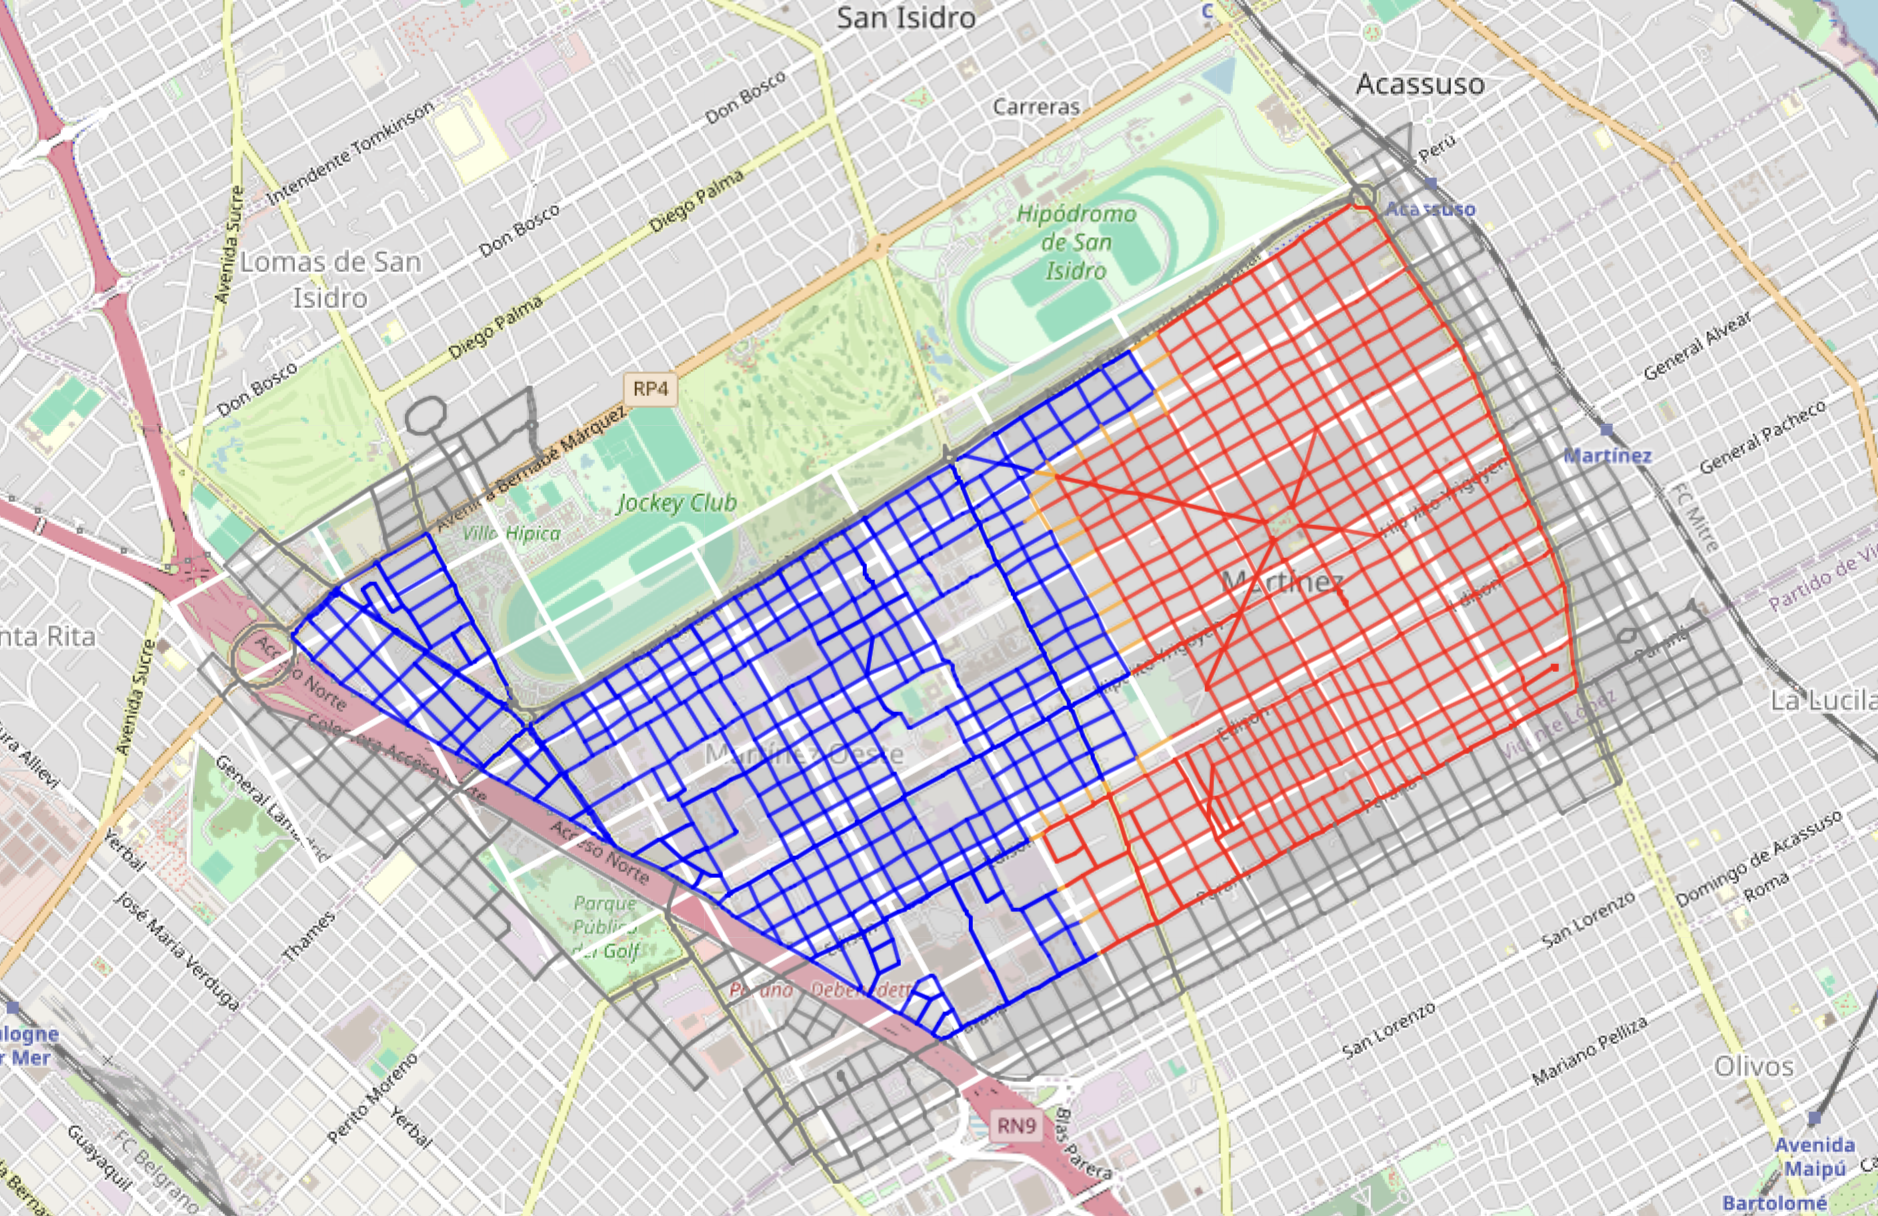
\includegraphics[scale=0.3]{img/zonas_martinex.png}
    \caption{Zonificación}
    \label{fig:zone}
\end{figure}


Similar al modelo principal, vamos a pensar a las calles como aristas y las intersecciones como nodos. Primero tenemos que pensar en cual es la función objetivo de este nuevo modelo. Vamos a querer minimizar la distancia máxima entre los nodos de una zona para poder lograr la forma compacta que buscamos. A través de restricciones flujo vamos a lograr que sean zonas conexas y usando otras restricciones auxiliares vamos a asignar cada nodo a una zona.

\newpage

Dado un grafo $G = (V,E)$,  $d:E\rightarrow \mathbb{R}$ como la distancia de un eje, $q:V\rightarrow \mathbb{R}$ como la demanda de un nodo, $U$ como una cota superior sobre la demanda calculada como $\frac{D_T}K$, es decir, la demanda total sobre la cantidad de zonas. $W$ como la capacidad del camión y $K$ como la  cantidad de zonas que debemos definir, vamos a precisar de las siguientes variables:

\begin{align*}
    X_{ui} &= 
    \begin{cases}
        1 & \text{si el nodo } u \text{ representa la zona } i \\
        0 & \text{caso contrario}
    \end{cases} \\
    Z_{ui} &= 
    \begin{cases}
        1 & \text{si el nodo } u \text{ es asignado a la zona } i \\
        0 & \text{caso contrario}
    \end{cases} \\
    Y_{uv} &= 
    \begin{cases}
        1 & \text{si los nodos } u \text{ y } v \text{ son asignados a zonas distintas}\\
        0 & \text{caso contrario}
    \end{cases} \\
    F_{ij} &= \text{Flujo del eje } ij \\
    D_i &= \text{Distancia máxima de la zona } i
\end{align*}

\begin{align}
    \min \quad & \sum^K_{i=1} D_i \\
    \text{sujeto a} \quad & \sum^K_{i=1} X_{ui} = 1 & \\
    & X_{ui} - X_{vi} \leq Y_{uv} & \forall i = 1\dots k \text{ } \forall (u,v) \in E\\
    & X_{vi} - X_{ui} \leq Y_{uv} & \forall i = 1\dots k \text{ } \forall (u,v) \in E\\
    & X_{ui} + X_{vi} + Y_{uv} \leq 2 & \forall i = 1\dots k \text{ } \forall (u,v) \in E\\
    & \sum_{u\in V} Z_{ui} = 1 & \forall i=1\dots k \\
    & Z_{ui} \leq X_{ui} & \forall i=1\dots k \text{ } \forall u \in V\\
    & F_{uv} + F_{vu} \leq M(1 - Y_{uv}) & \forall (u,v) \in E \\
    & \sum_{v \in \delta^-(u)} F_{uv} - \sum_{v \in \delta^+(u)} F_{uv} \geq 1 - M\sum^K_{i=1}Z_{ui} &\forall u \in V \\
    & D_i \geq d_{uv} (X_{ui} + X_{vi} - 1) & \forall i = 1\dots k \\
    & \sum_{u\in V} X_{ui} q_u \geq 0.9 W & \forall i = 1\dots k \\
    & \sum_{u\in V} X_{ui} q_u \leq 1.05 U & \forall i = 1\dots k \\
    & \sum^K_{i = 1} D_i \geq \frac{K}{1.05} D_i & \forall i = 1\dots k \\
    & \sum^K_{i = 1} D_i \leq \frac{K}{0.95} D_i & \forall i = 1\dots k
\end{align}

En la restricción $(14)$ forzamos a que un nodo se encuentre únicamente en una zona. En las restricciones $(15)$, $(16)$ y $(17)$ relacionamos las variables $X$ e $Y$ de forma de establecer una restricción de asignación de zona a cada para de nodos. Luego en la $(18)$ elegimos un único representante por zona y en la $(19)$ nos aseguramos de que ese representante efectivamente esté asignado a la zona que representa. En $(20)$ y $(21)$ establecemos el flujo que debe haber entre nodos. En la $(22)$ asignamos la distancia máxima de cada zona. En la $(23)$ y $(24)$ restringimos a la zona contra la capacidad del camión para que sea posible recorrerla recolectando en un único viaje. Además, junto a $(25)$ y $(26)$ hacemos que las $K$ zonas sean balanceadas en demanda y distancia.

\chapter{Construcción de Instancias}
\section{Sistemas de Información Geográfica}

Un \textit{sistema de información geográfica} (SIG) es un conjunto de herramientas que integra y relaciona diversos componentes que permiten la organización, almacenamiento, manipulación y análisis de grandes cantidades de datos procedentes del mundo real que están vinculados a una referencia espacial.

\vspace{3mm}

Para obtener la información que nos interesa de un mapa, como calles, coordenadas de esquinas, etc., debemos utilizar un servicio de geolocalización como \textit{Google Maps}. Sin embargo, este no nos proporciona toda la información que necesitamos, por lo tanto, usaremos \textit{Open Street Map (OSM)}, un proyecto colaborativo de origen británico para crear mapas editables y libres.

\vspace{3mm}

Dado que las zonas de San Isidro no son rectángulos, más bien son polígonos, tuvimos que generar primero estas figuras utilizando archivos \textit{geojson}, los cuales son archivos \textit{json} con una estructura predefinida específica para contextos geográficos. Por otro lado, no queremos únicamente el polígono de la zona a recorrer, si no que también queremos los alrededores para poder darle la posibilidad al camión de salir de la zona y volver a entrar simulando movimientos permitidos en la realidad. Con lo cual, tendríamos un polígono extendido ligado a una zona, el cual contiene la zona y sus alrededores. Luego a través de una API brindada por \textit{OSM} podemos obtener el mapa con todos los detalles del polígono utilizado.

\section{Transformando Mapas en Grafos}

Una vez generado el mapa \textit{OSM} vamos a querer manipularlo para poder retener únicamente la información que nos importa y agregarle datos adicionales que no se encuentran en \textit{Open Street Maps} que nos brindaron del Municipio. Resumiendo, de cada calle queremos saber si:
\begin{itemize}
    \item Estamos obligados a recorrerla recolectando residuos.
    \item Si es mano única o doble.
    \item Forma parte de un barrio privado o informal.
    \item Si es una calle de empedrado.
    \item Si una de sus esquinas es un cruce ferroviario.
    \item Si una de sus esquinas tiene un semáforo y si este tiene giro a la izquierda.
\end{itemize}

Para ello vamos a filtrar el mapa \textit{OSM} quedándonos con los elementos que tienen cierto \textit{keyword} identificándolos como una calle para poder generar el grafo mixto $G$ modelando las intersecciones como nodos y las calles como aristas. Por lo tanto, generaríamos un grafo $G = (V, E \cup A)$ donde $E$ es el conjunto de aristas y $A$ el conjunto de arcos.

\vspace{3mm} 

Sea $C$ el conjunto de calles del mapa \textit{OSM}. El proceso para filtrar el mapa se basa en analizar cada $c\in C$, para ello comenzamos separando en obligatorias o no usando la librearía de python, \textit{shapley}, con la cual podemos verificar si un punto está dentro de un polígono en el mapa. Luego, conociendo las esquinas de la calle $c$ que estamos analizando las vamos a agregar al conjunto de nodos $V$ marcando si tiene alguna característica de interés como cruce de tren, semáforo con o sin luz de giro, etc. 

\vspace{3mm}
Para realizar esta decisión debemos comparar coordenadas, ya que es la única información en común entre las esquinas del mapa \textit{OSM} y el dataset brindado por el municipio. Luego, dada una lista de puntos $A$ y una esquina candidata $e$, queremos determinar si existe $a \in A$ tal que $e$ corresponda al mismo punto que $a$.

\vspace{3mm}

Para verificar si dos coordenadas representan la misma esquina utilizamos la distancia euclídea, considerando que $|a - e|_2 < \epsilon$. No buscamos igualdad exacta ya que, al tratarse de coordenadas geográficas, pueden existir pequeñas diferencias en su representación para una misma esquina en distintos mapas o datasets.

\vspace{3mm}

Para resolver este pequeño problema vamos a pensar la lista de coordenadas como una matriz $A$ donde cada fila es una coordenada del dataset. A cada fila le vamos a restar el punto $e$ generando una matriz $A'$.Luego, siendo $A'_i$ la $i$-ésima fila de $A'$, vamos a corroborar que $\min_{i=1,\dots,n}(\|A'_i\|_2) < \epsilon$. 

Esta operación puede implementarse de manera muy eficiente utilizando \textit{NumPy}, ya que la resta del punto $e$ a todas las filas de la matriz y el cálculo de las normas pueden realizarse mediante operaciones vectorizadas. Estas permiten aplicar una misma operación a todos los elementos de un arreglo de manera simultánea, evitando iteraciones explícitas y aprovechando implementaciones optimizadas de bajo nivel.

\vspace{3mm} 

Una vez filtrado el mapa vamos a eliminar las calles que no podemos recorrer. Estas calles son las que no tienen salida, ya que el camión no puede dar un giro en U en este tipo de calles. Para ello vamos a eliminar los nodos tal que pertenezcan a alguno de los siguiente 3 conjuntos, una vez eliminados, vamos a volver a generar estos conjuntos y repetir el proceso hasta que al volverlos a generar estén los 3 vacíos.

\begin{itemize}
    \item $I = \{v\in V: d^+(v) = 0\}$
    \item $O = \{v\in V: d^-(v) = 0\}$
    \item $U = \{v\in V: d^+(v) = d^-(v) = 1 \land \exists u\in V : uv,vu \in E\}$
\end{itemize}

El conjunto $I$ representa las intersecciones inaccesible para nosotros, generado en consecuencia de que estamos tomando un polígono el cual deja calles afuera, en particular, calles que conectan puntos fuera del polígono con los que están dentro. Luego, el conjunto $O$ representa intersecciones parecidas a las de $I$, salvo que son para el otro sentido, es decir, son las que conectan puntos de nuestro polígono con los puntos fuera de el. Finalmente, el conjunto $U$ son las verdaderas calles sin salida que se encuentran en la ciudad.

\vspace{3mm} 

El siguiente paso es calcular los costos de cada arista o arco, tiempo, dist, demanda...

\vspace{3mm} 

Otro dato de interés son las curvas, ya que queremos minimizar la cantidad de curvas tomadas por el camión. Para identificar las curvas vamos a utilizar los nombres de cada calle, con lo cual, dadas 3 intersecciones, $u,v$ y $w$, estando parados en la intersección $v$, viniendo de la calle que une las intersecciones de $u$ a $v$, continuando por la calle que une $v$ y $w$, vamos a marcar como curva el recorrido $uvw$ si y sólo si los nombres de las calles que unen las intersecciones difieren.
\vspace{3mm} 

Continuando con las curvas, además de marcarlas, vamos a identificar cuales son curvas a la izquierda y si están prohibidas. Para ello, vamos a analizar las triplas para las cuales la calle que une la intersecciones $u$ y $v$ es doble mano o una avenida sin semáforo para girar a la izquierda. Una vez tenemos el conjunto de candidatas, vamos a calcular el ángulo orientado en sentido horario que generan y si este este pertenece al intervalo $[\textit{threshold} \pi]$ lo consideraremos como un giro a la izquierda ilegal.

\vspace{3mm} 

En la siguiente figura podemos visualizar el mapa \textit{OSM} filtrado, donde las calles de color \textit{amarillo} son las calles obligatorias de recorrer, las \textit{azules} son las calles empedradas y las \textit{grises} son las no obligatorias.


\begin{figure}[h!]
    \centering
    \begin{minipage}{0.48\textwidth}
        \centering
        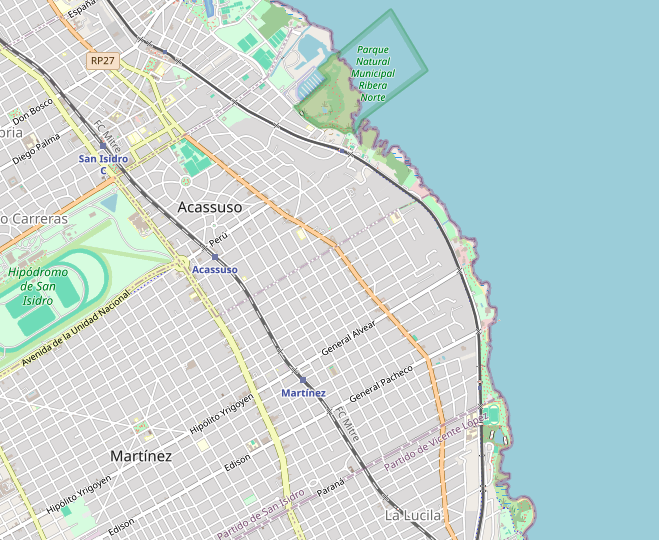
\includegraphics[width=\textwidth]{img/AcassusoReal.png}
        \caption{Acassuso \textit{OSM}}
        \label{fig:imagen1}
    \end{minipage}
    \hfill
    \begin{minipage}{0.48\textwidth}
        \centering
        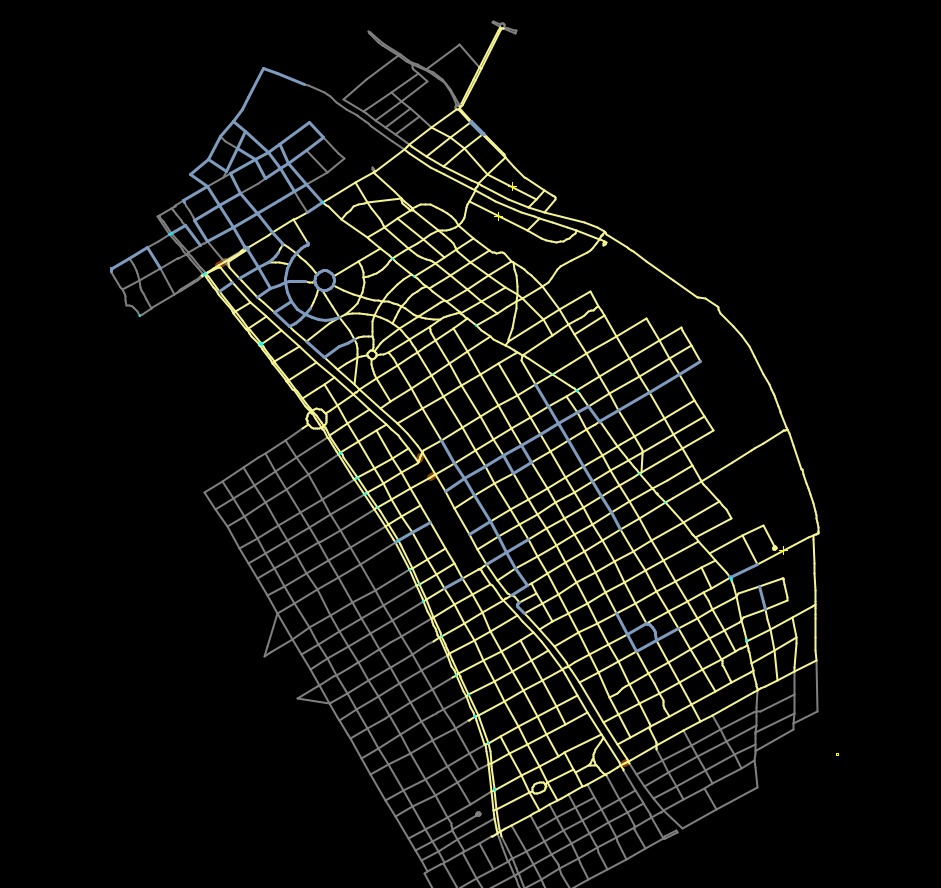
\includegraphics[width=\textwidth]{img/AcassusoOSM.jpeg}
        \caption{Acassuso \textit{OSM} Filtrado}
        \label{fig:imagen2}
    \end{minipage}
\end{figure}

Recapitulando, a partir de un polígono generamos un una instancia del problema donde tenemos el grafo $G = (V, E\cup A)$, es decir el área a recolectar, y 2 funciones $t:E\cup A\rightarrow \mathbb{R}$ y $d:E\cup A\rightarrow \mathbb{R}$ que representan, para todo eje perteneciente a $G$, el costo en tiempo (seg) de recorrerlo y la demanda de basura del mismo respectivamente.


\subsection{Zonificando con Grillas}

Para poder zonificar el grafo en $k$ debemos procesar el mapa como fue explicado anteriormente. En un principio, no tuvimos problemas con el modelo, sin embargo, a medida que lo fuimos probando con instancias reales, el modelo comenzó a demorar mucho más de lo esperado. El objetivo de la zonificación era obtener un resultado concreto y rápido para que luego el modelo de optimización de recorridos encuentre la solución óptima.

\vspace{3mm}

Llegamos a la conclusión que estábamos entrando muy en detalle utilizando todos las intersecciones y calles del área para asignarles una zona. Para este problema auxiliar no queríamos una solución óptima de la distribución de calles, necesitábamos una solución eficaz y eficiente. Por lo tanto, decidimos separar el mapa en una grilla, donde cada celda contendría un conjunto de calles e intersecciones y representaría un nodo en el modelo, reduciendo los nodos un 98$\%$ y las aristas un 93$\%$ en promedio. [CHEQUEAR PORCENTAJES] 

\vspace{3mm}

El primer paso para generar la grilla es tomar las coordenadas extremas en latitud y longitud. A partir de este paso ya tenemos una grilla que contiene todos los nodos y aristas del grafo. Sin embargo, como el mundo no es perfecto, las calles de nuestra ciudad no están perfectamente alineadas con la latitud o la longitud, con lo cual, vamos a tener que rotar la grilla.

\vspace{3mm}

Para poder rotar la grilla necesitamos tener un ángulo de rotación, para ello, necesitamos formar un triangulo en nuestro mapa, donde el \textcolor{blue}{hipotenusa} quede alineado con una calle seleccionada previamente para alinear la grilla y el \textcolor{green!50!black}{cateto 2} paralelo a la longitud. Una vez generado el triángulo basta obtener el ángulo entre el \textcolor{red}{cateto 1} y la \textcolor{blue}{hipotenusa} para saber cuanto necesitamos girar la grilla. Una vez que tenemos el ángulo vamos a utilizar el método de \textbf{Givens} usado para rotar matrices $4\times4$ para rotar nuestra grilla y alinearla a las calles de la zona.

[DECIR QUE LA DISTANCIA SE CALCULA DE OTRA MANERA EN LA TIERRA?]

\begin{figure}[h!]
    \centering
    \begin{minipage}{0.48\textwidth}
        \centering
        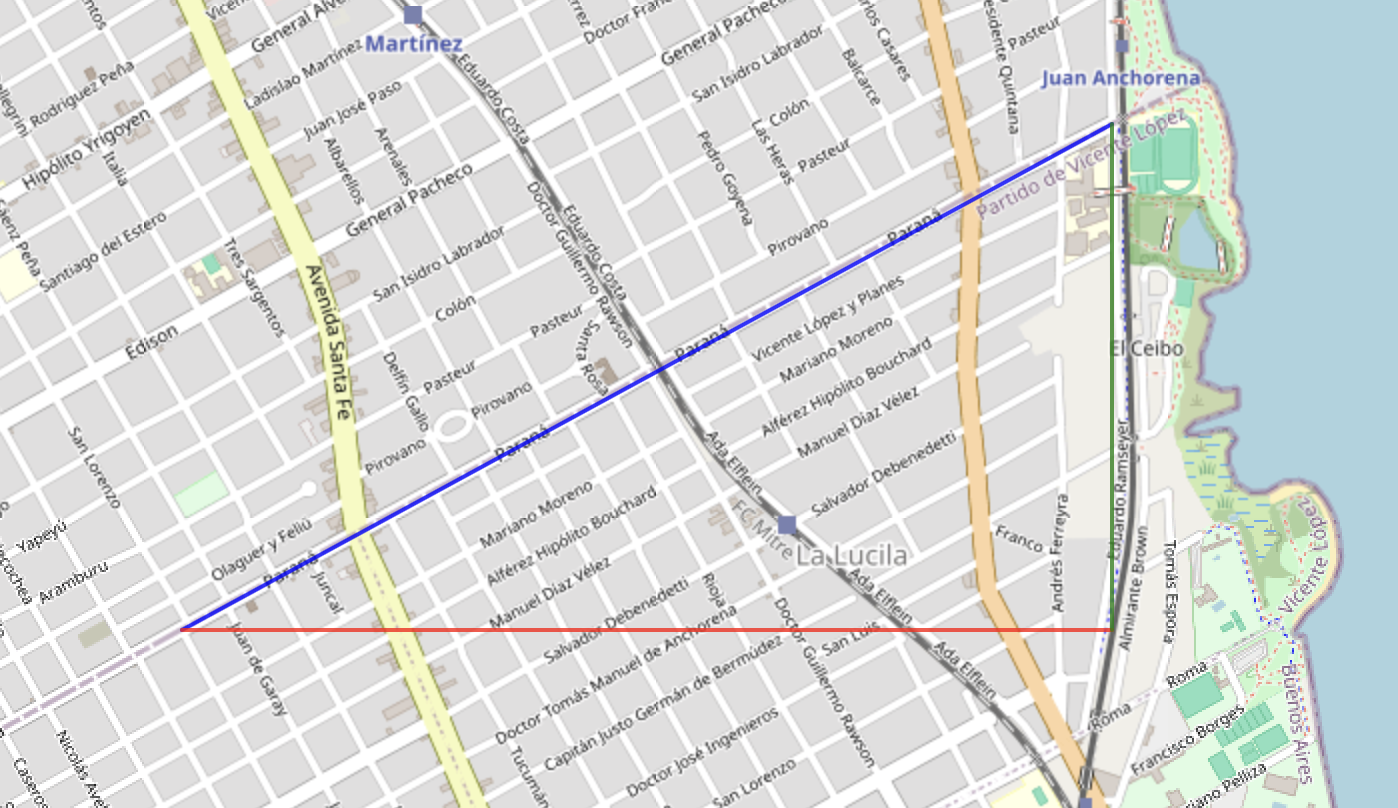
\includegraphics[width=\textwidth]{img/triangulo.png}
        \caption{Triángulo de rotación}
        \label{fig:triangulo}
    \end{minipage}
    \hfill
    \begin{minipage}{0.48\textwidth}
        \centering
        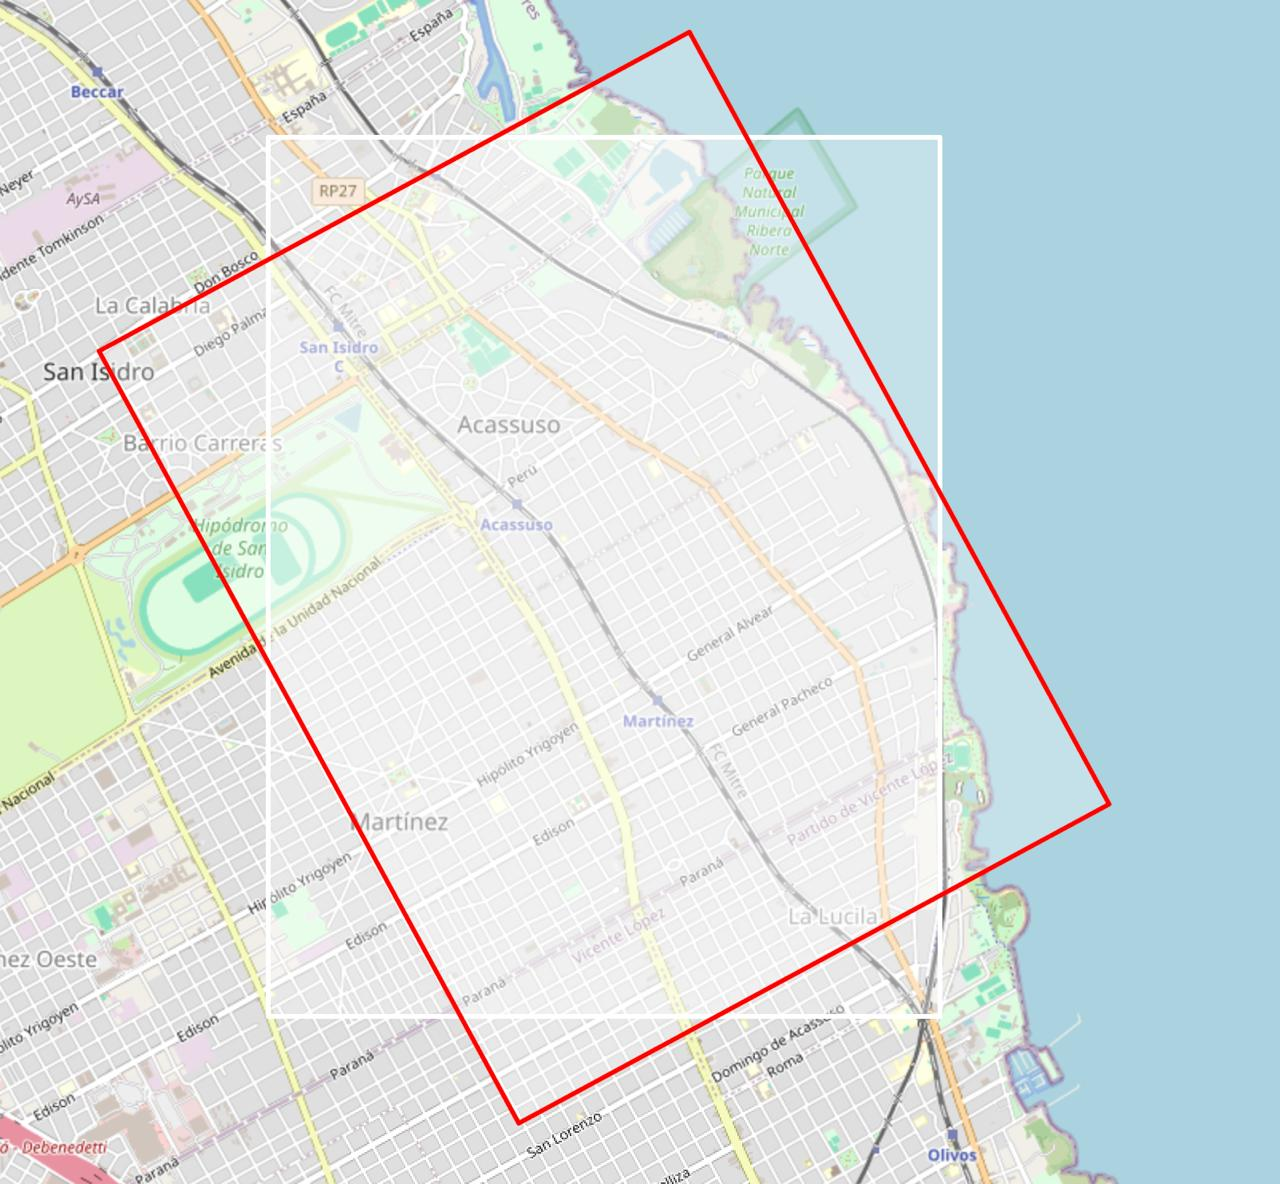
\includegraphics[width=\textwidth]{img/grilla_rotada.jpeg}
        \caption{\textcolor{red}{Grilla rotada} vs Grilla original}
        \label{fig:imagen2}
    \end{minipage}
\end{figure}


El siguiente paso es generar las celdas, para ello, a través de un parámetro externo sobre la máxima cantidad de celdas, dividimos equitativamente la grilla para obtener lo más parecido a este parámetro. Luego, debemos iterar celda por celda para poder calcular la demanda de cada una de ellas con la siguiente fórmula:
$$
D(C) = \sum_{(u,v) \in E \space \land \space (u,v) \in C} d((u,v))
$$

Esto se traduce a decir que la demanda $D$ de cada celda $C$ es la sumatoria de la demanda $d:E\rightarrow \mathbb{R}$ de toda arista $(u,v)$ que se encuentra dentro de la celda.

\vspace{3mm}

Finalmente obtuvimos una grilla la cual podemos traducir a un grafo grilla con demanda por nodo y distancia entre ellos calculada desde el centro de cada grilla.



\chapter{Construcción de Soluciones}
\section{Transformando Grafos en Recorridos}

Una vez finalizado el procesamiento del mejor recorrido obtenemos una asignación de cada calle a un camión en particular. Con lo cual, sabemos que calles recorre ese camión, donde comienza el recorrido y que su recorrido es un circuito, es decir termina donde comienza, en el depósito.

\vspace{3mm}

Para armar el recorrido final uno pensaría que basta con concatenar las calles asignadas a un mismo camión. Sin embargo, no cualquier concatenación de calles nos deja con un circuito como el que queremos.

\vspace{3mm}

Vamos a querer encontrar circuitos eulerianos en cada región, donde una región son las calles que debe recorrer el camión. Para ello, vamos a ir consumiendo aristas partiendo desde el depósito, donde cada nodo tiene igual grado de entrada que de salida, asegurandonos un circuito. Siempre que el nodo tenga una única entrada y una única posible salida la decisión es trivial, el problema surge cuando ese número es mayor a 1. En este caso, sabemos que va a haber solución pero tenemos que tomar la decisión si continuar por la misma vía o cambiar de vía haciendo que el camión gire en la realidad.

\vspace{3mm}

C

\chapter{Experimentos y Resultados}

\chapter{Conclusiones y próximos pasos}

%%%% BIBLIOGRAFIA
\backmatter
%\bibliography{tesis}

\end{document}
